% Copyright (C) 2012 Thomas L. Kula
% All Rights Reserved
%
% See the file LICENSE for license terms.
\documentclass[12pt]{article}
\usepackage{graphicx}
\usepackage{rotating}
\usepackage{fix-cm}
\usepackage{multirow}
\setlength{\paperwidth}{5.5in}
\setlength{\paperheight}{8.5in}
\setlength{\textheight}{7.45in}
\setlength{\topmargin}{-1.0in}
\setlength{\oddsidemargin}{-0.5in}
\setlength{\evensidemargin}{-0.5in}
\setlength{\textwidth}{4.0in}
\setlength{\parindent}{0in}
\setlength{\parskip}{3mm}
\usepackage[print]{booklet} \nofiles
\source{\magstep0}{5.5in}{8.5in}
\target{\magstep0}{11in}{8.5in}
\setpdftargetpages
\pagestyle{empty}
\begin{document}


\begin{center}
{\fontsize{36}{48}\selectfont \textsc{Haiku a Day }}
\end{center}

\vspace*{3.5cm}

{\fontsize{20}{40}\selectfont 

Polka in my mind 

In an endless loop, dancing 

Roll out the barrel


}

\vspace*{5.0cm}
\begin{center}
{\large{Issue 83: May 2012}} \\[5mm]
{\fontsize{8}{8}\selectfont  \textsc{ St. Joshua Norton Press }} \\[1mm]
{\fontsize{6}{6}\selectfont Mathom House by the Cloisters \textbar The People's Republic of Ames }
\end{center}


\newpage

I'm happy to report that May made me an uncle, to one
Meghan Elizabeth Kula. I'm looking forward to spoiling
her.

--- Thomas

http://kula.tproa.net/had/ \\
kula@tproa.net

Download this and previous HADs at the website, so you can
print out your own (DIY, yeah!) or if you want me to send
you one, send me your address, and maybe a stamp if you
are feeling nice. Or send me something you've made ---
trades always appreciated, postcards are nice too.

\vfill

1 May 2012

Walking down Broadway \\
A few thousand friends in tow \\
Making me feel good

2 May 2012

I hear a faint call \\
Tom Collins in the distance \\
I wait for summer

3 May 2012

That cucumber has \\
Been in the fridge for too long \\
Into the garbage

\newpage

4 May 2012

Hurried, in three stores \\
To find the stuff to make pie \\
I am exhausted

5 May 2012

Cinco de Mayo \\
Seems weird until I think of \\
The Fourth of July

6 May 2012

Blankets, what a word \\
Even the name feels like it \\
Wraps you in a hug

7 May 2012

More avocados, \\
Is my theory from here out; \\
Crave guacamole

8 May 2012

Bottom of the bag \\
Bits and crumbs, sad, out of place \\
Chip effluvia

9 May 2012

With light just breaking \\
I stand before the morning \\
Ready for the day

10 May 2012

Last light banked below \\
Shadows as blankets draw closer \\
Ready for the night


\newpage

11 May 2012

Glory eternal \\
Consider the falafel \\
The joy that it brings

12 May 2012

What was I thinking? \\
Late night cravings leading to \\
Dishes of Ghastly

13 May 2012

Late night boredom turns \\
Reveals, hidden, a mission: \\
Cross the Brooklyn Bridge

14 May 2012

A random day off \\
Productivity Promise, \\
Really Laziness

15 May 2012

From down the street comes \\
A tinny little tune, bright \\
Promise of ice cream

16 May 2012

``Congratulations'' --- \\
I say again and again --- \\
``Now sit the hell down.''

17 May 2012

Pitcher in the Sun \\
Full of cold iced tea, glistens \\
Noble refreshment


\newpage

18 May 2012

Never staying still \\
Ill-fitting bed sheets: bonkers \\
Unfolded slumber

19 May 2012

Hidden is growing \\
Recycling under the sink \\
Nothing, then explodes

20 May 2012

A tiny insect \\
Wanders down from the river \\
To land on my hand

21 May 2012

Deep in the belly \\
Of the thing that will consume; \\
I forget to lunch

22 May 2012

If a clean desk is \\
A sign of insanity \\
I'm perfectly sane

23 May 2012

An endless circle \\
Running that takes all the time \\
And running, makes time

24 May 2012

Rocking and creaking \\
Bits falling off left and right \\
I still keep the chair


\newpage

25 May 2012

A call late at night, \\
Holy Fuck I'm an Uncle \\
Meghan joins the world

26 May 2012

Late night, up running \\
Means a rough start next morning \\
Give me some coffee

27 May 2012

Brunch: standing in line \\
A long wait, going elsewhere \\
Tasty food follows

28 May 2012

The long path tonight \\
Simple joy, meandering \\
No hurry for home

29 May 2012

Softly the bird flits \\
Lands, bending a stalk of grass \\
Butterfly annoyed

30 May 2012

Soft dusty exhale \\
A warm breath growing colder \\
Air conditioner

31 May 2012

A constant nagging \\
Bit of thread, unraveling \\
Unknits sanity

\newpage

\begin{center}
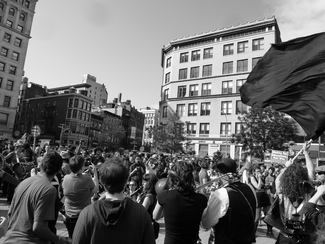
\includegraphics[width=325pt]{may-day.png}

May Day 2012 \\
Union Square, New York City
{\tt kula.tproa.net/photos/2012/2012-mayday/ }

\end{center}

\newpage

\thispagestyle{empty}
\vspace*{12cm}
\begin{sideways}
\Large{St. Joshua Norton Press}
\end{sideways}
\begin{sideways}
\Large{PO Box 250138}
\end{sideways}
\begin{sideways}
\Large{New York NY 10025}
\end{sideways}


\end{document}


